%!TEX root = ../thesis.tex
\chapter{Experimental Results} \label{chap:exp-results}

\section*{}

In order to reliably validate the defect probability prediction we used an existing database of faults, \emph{Defects4J}.
This database contains a list of commits with defects and their location from five different projects (JFreechart, Closure compiler, Apache commons-lang, Apache commons-math and Joda-Time).
Since compatibility with \emph{Barinel} and using \emph{Git} is required, only the last three projects were used, making a total of 184 commits.
%
\begin{table}[H]
	\centering
	\begin{tabular}{|l|l|l|}
	\hline
	\textbf{Project name} & \textbf{Shortname} & \textbf{Defects} \\ \hline
	Apache commons-lang   & Lang               & 59               \\ \hline
	Apache commons-math   & Math               & 101              \\ \hline
	Joda-Time             & Time               & 25               \\ \hline
	\end{tabular}
	\caption{Test Set}
	\label{test-set}
\end{table}

\section{Estimating Defect Probability}

First we must know the characteristics of each project in order to better interpret the results, so a table was made containing information about the first and last commit of each
project.
%
\begin{table}[H]
\centering
\begin{tabular}{|l|l|l|l|l|l|}
\hline
\textbf{Project} & \textbf{Defect} & \textbf{Files} & \textbf{Previous commits} & \textbf{Previous fix commits} & \textbf{Contributors} \\ \hline
Lang             & 1               & 108            & 3569                      & 366                           & 40                    \\ \hline
Lang             & 59              & 81             & 1533                      & 190                           & 25                    \\ \hline
Math             & 1               & 813            & 4877                      & 564                           & 28                    \\ \hline
Math             & 103             & 370            & 957                       & 66                            & 15                    \\ \hline
Time             & 1               & 162            & 1717                      & 234                           & 27                    \\ \hline
Time             & 26              & 733            & 1474                      & 195                           & 9                     \\ \hline
\end{tabular}
\caption{Examples of project states from the test set}
\label{test-set-examples}
\end{table}

Three different classification algorithms were tested: Support Vector Machines, Random Forests and AdaBoost.
Our preliminary tests showed that Random Forests is the algorithm that provides an higher accuracy, that using the normalized values didn't help and the best label to use for training is \code{_mostChanged}, so we will focus on this test case.

Figures \ref{fig:clean-dp-count} and \ref{fig:buggy-dp-count} illustrate the different defect probabilities distributions of faulty and probably clean components, across all the 184 defects, respectively.
%
\begin{figure}[!]
  \begin{center}
    \leavevmode
    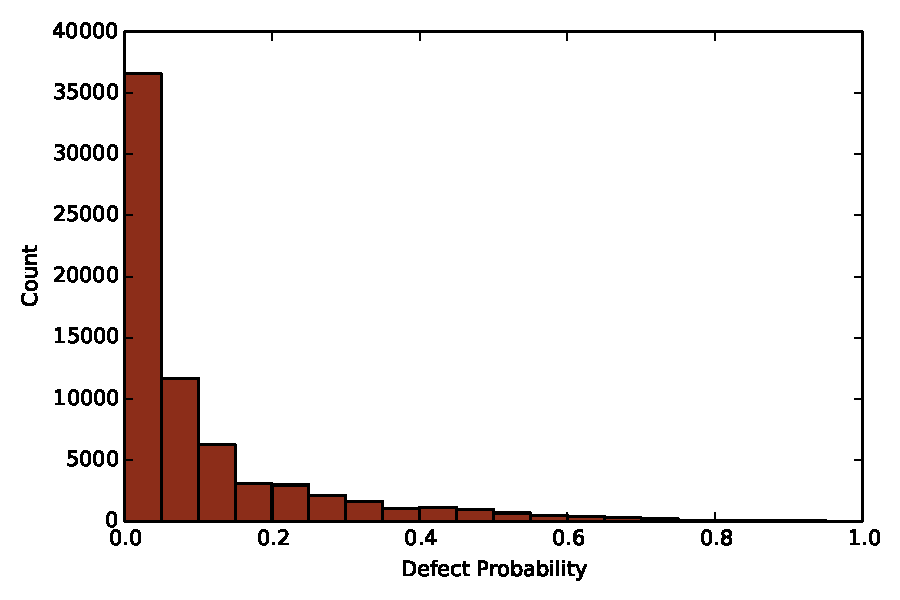
\includegraphics[width=0.6\textwidth]{clean-dp-count.pdf}
    \caption{Distribution of predicted defect probabilities for probably clean components}
    \label{fig:clean-dp-count}
  \end{center}
\end{figure}
%
\begin{figure}[!]
  \begin{center}
    \leavevmode
    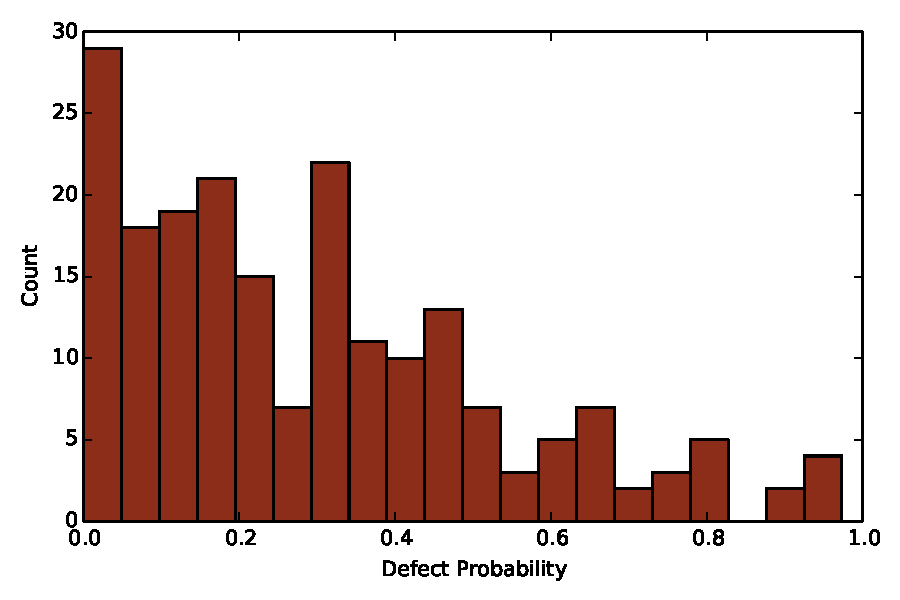
\includegraphics[width=0.6\textwidth]{buggy-dp-count.pdf}
    \caption{Distribution of predicted defect probabilities for faulty components}
    \label{fig:buggy-dp-count}
  \end{center}
\end{figure}
%
However since we want the faulty component to be the one with the highest defect probability, it is important not only to verify the defect probability for the faulty component, but also to compare it to the probabilities of the other, probably clean, components in the project. Figure \ref{fig:dp-count} illustrates a case where the faulty component has a low defect probability, $12\%$, but it still is on the top $17\%$.
%
\begin{figure}[!]
  \begin{center}
    \leavevmode
    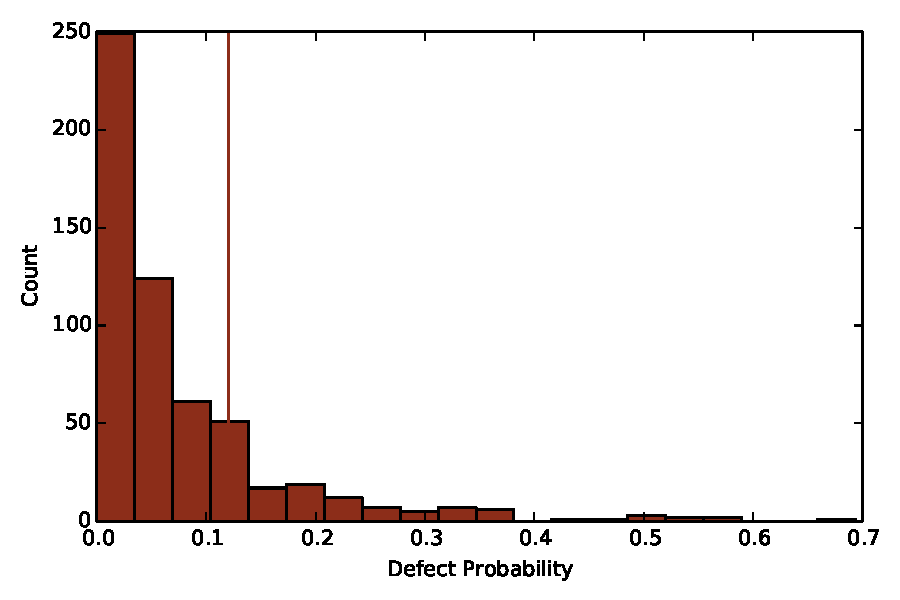
\includegraphics[width=0.6\textwidth]{dp-count_math050.pdf}
    \caption{Histogram of predicted defect probabilities for Project Math (Defect 50), with a vertical line identifying the faulty component prediction}
    \label{fig:dp-count}
  \end{center}
\end{figure}

Figure \ref{fig:dp-faults-position} exhibits the relative position of the faulty component for all the 184 defects and allowed to concluded that the average percentage of components with higher defect probability than the faulty component is just $16.6\%$ and the median is $10.6\%$.

\begin{figure}[!]
  \begin{center}
    \leavevmode
    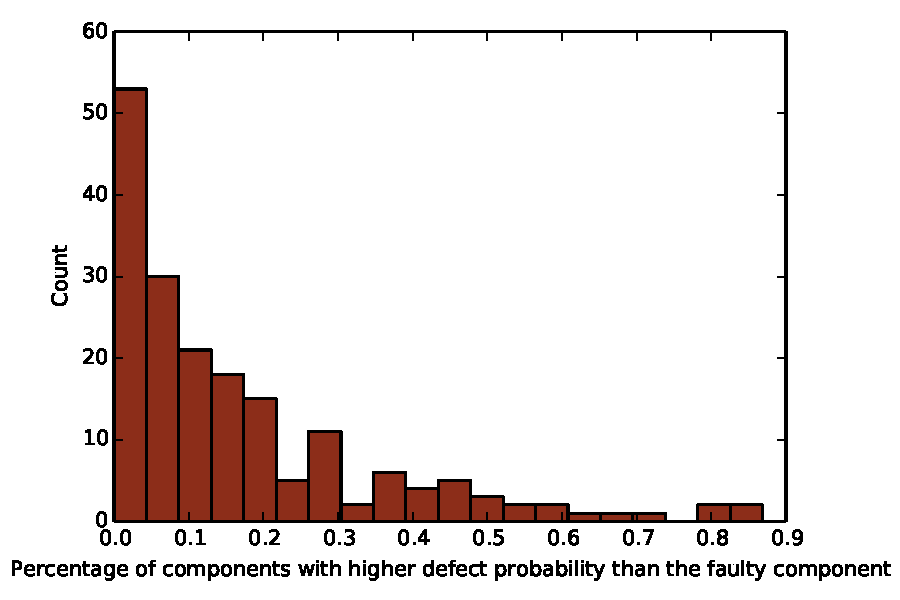
\includegraphics[width=0.6\textwidth]{faults-position.pdf}
    \caption{Histogram of the percentage of components with higher defect probability than the faulty component for all 184 defects}
    \label{fig:dp-faults-position}
  \end{center}
\end{figure}

% GUIDELINES
% SVM vs Random Forests vs AdaBoost
% Relation between the value calculated for the wanted faulty classes vs others
% Example for one project (histogram of prediction. Vertical line - faulty) If more than one faulty use the higher predicted value
% Histogram for percentage positions of these faulty components


\section{Barinel Integration}

% Present the best possible results
% Present the results with 10% better or 10% worse
% Distribution of positions

Two types of integration with Barinel were tested so the results will be presented separately in the following two sub-chapters. However, in the interest of better understanding the results, an analysis of the results of the unmodified Barinel was made.

The unmodified Barinel analysis, represented on figure \ref{fig:fault-positions}, showed that on $44.57\%$ of the 184 project states the faulty component already are on the first position and on $5.98\%$ it has associated a $0\%$ probability of being faulty. So, no improvements can be made on $50.55\%$ of the examples of the test set. It also showed that in $88.04\%$ of the results the component with the defect is above the 10th position. For the sake of this analysis, in case of draw, we consider the best position and won't consider on the graphics the cases where the associated probability is $0\%$.

\begin{figure}[!]
  \begin{center}
    \leavevmode
    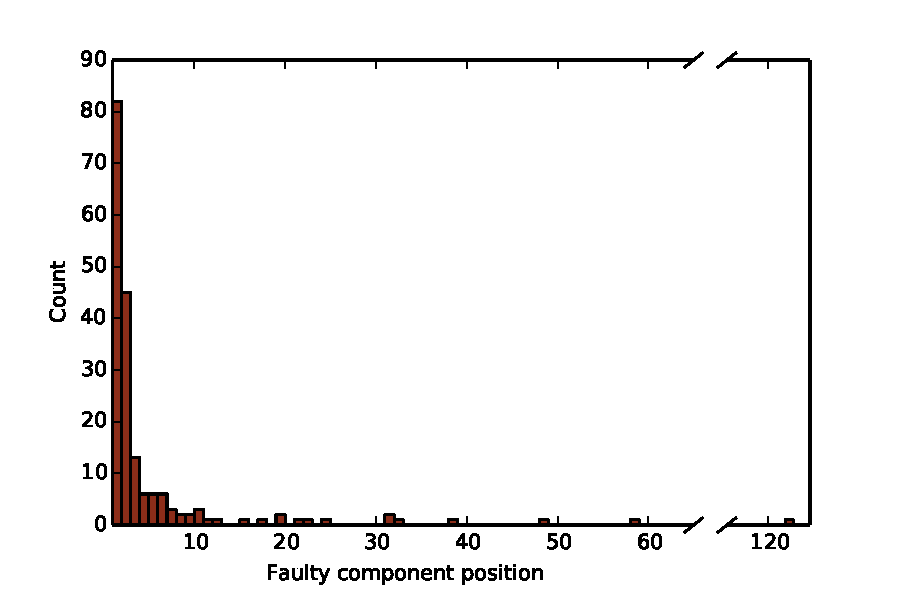
\includegraphics[width=0.6\textwidth]{unmodified-barinel_positions.pdf}
    \caption{Histogram of the relative position of all faulty components, with a probability above zero, reported by the unmodified barinel}
    \label{fig:fault-positions}
  \end{center}
\end{figure}


\subsection{Results Modification}

First, to be able to contextualize the results, the best and worst scenarios were tested. If the predicted defect faulty was 1 to all the faulty components and 0 for all the others, there would be an improve on 37 cases. If, for instance, the probabilities were totally wrong, it would worsen 54 cases.

Given the predicted defect probabilities is important to determine the best value to use as the minimum for a component to be considered possibly faulty. When considered possibly faulty, as explained in \ref{chap:barinel-integration}, the Barinel fault probability is doubled. For each value from $0.5$ to $1$, at $0.05$ steps, the gain, loss and delta was calculated, as we can see in \ref{fig:results-modification}.

\begin{figure}[!]
  \begin{center}
    \leavevmode
    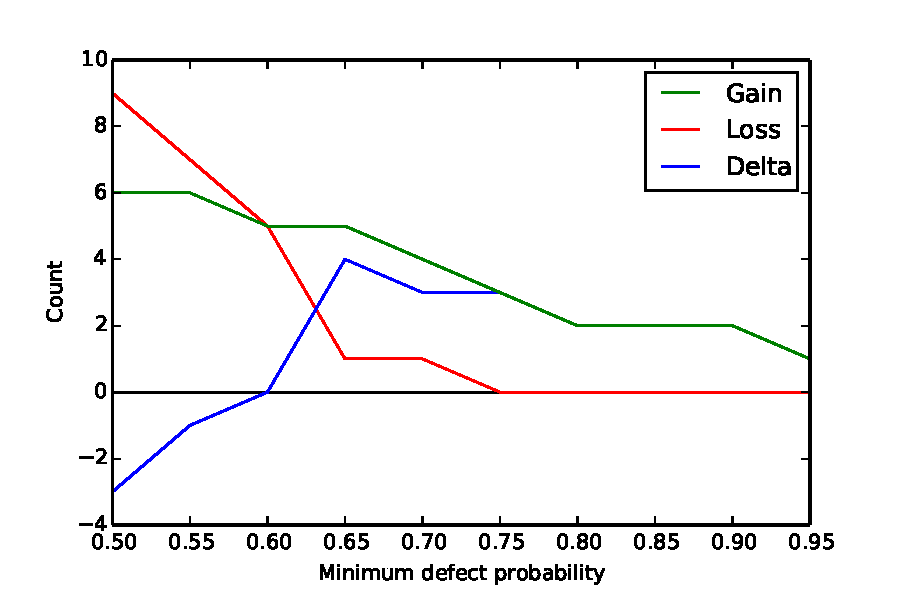
\includegraphics[width=0.6\textwidth]{barinel-integration-1.pdf}
    \caption{Results modification effect on Barinel results, by minimum defect probability}
    \label{fig:results-modification}
  \end{center}
\end{figure}


\subsection{Priors Replacement}

\todo{... Waiting ... Flaky tests ...}